% Common packages pre-cached at image build time so they work without network access.
\documentclass{article}
\usepackage[utf8]{inputenc}
\usepackage[T1]{fontenc}
\usepackage{lmodern,microtype,mathtools,amsthm,siunitx,physics}
\usepackage{graphicx,float,wrapfig,subcaption,caption}
\usepackage{booktabs,multirow,tabularx,longtable,array}
\usepackage{tikz,pgfplots}
\usepackage{listings,algorithm,algpseudocode}
\usepackage{natbib,url,hyperref,cleveref}
\usepackage{fancyhdr,setspace,geometry,enumitem,titlesec,lipsum,todonotes,xcolor}
\usepackage{amssymb,mathrsfs,bm,tcolorbox,csquotes,multicol,adjustbox,makecell,colortbl}
\usepackage{threeparttable,xspace,comment,appendix,authblk,pdfpages}
\usepackage[english]{babel}
\pgfplotsset{compat=1.18}
\begin{document}
\section{Warm-up}\lipsum[1]
\begin{tikzpicture}\draw (0,0) -- (1,1);\end{tikzpicture}
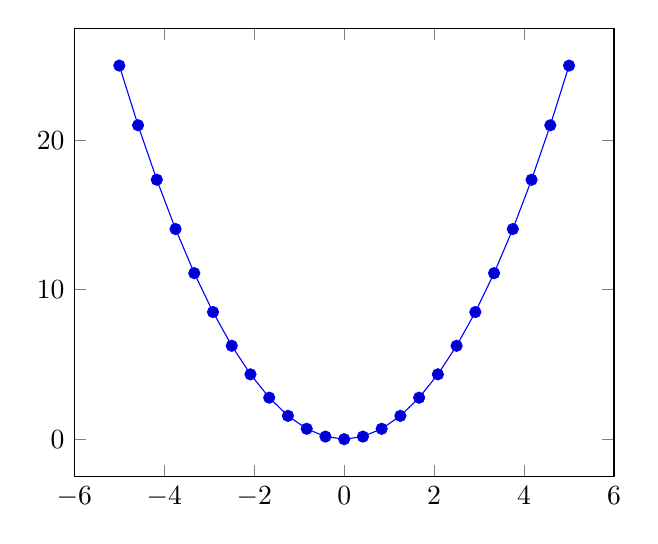
\begin{tikzpicture}\begin{axis}\addplot {x^2};\end{axis}\end{tikzpicture}
\begin{lstlisting}[language=Python]
print("hello")
\end{lstlisting}
\SI{3}{\metre} \todo{note}
\end{document}
